% 建议使用 XeLaTeX 或 LuaLaTeX 编译(中文与公式支持更佳)
\documentclass[UTF8,zihao=-4]{ctexart}

\usepackage[a4paper,margin=2.5cm]{geometry}
\usepackage{amsmath, amssymb, amsthm}
\usepackage{bm}
\usepackage{hyperref}
\usepackage{graphicx}
\usepackage{caption}
\usepackage{listings}
\usepackage{xcolor}
\usepackage{float}
\usepackage{placeins}
\graphicspath{{figures/}}

\lstdefinestyle{code}{
  basicstyle=\ttfamily\small,
  numbers=left,
  numberstyle=\tiny,
  numbersep=8pt,
  keywordstyle=\color{blue},
  commentstyle=\color{teal!70!black},
  stringstyle=\color{orange!70!black},
  showstringspaces=false,
  breaklines=true,
  frame=single,
  framerule=0.3pt,
  rulecolor=\color{black!15}
}
\lstset{style=code}

\title{层次聚类:原理、公式、应用与实战}
\author{}
\date{\today}

\begin{document}
\maketitle

\section{引言}
层次聚类通过不断合并或拆分簇来构建数据的多层次结构,无需预先指定簇数。常见的自底向上(凝聚式)方法先将每个样本视为独立簇,再依据链接准则(如最短距离、最长距离、平均距离或 Ward 距离)逐步合并最相近的簇。最终得到的树状图(dendrogram)记录了整个合并过程,可在不同高度切割以获得不同数量的簇。

\section{原理与公式}
\subsection{链接函数}
考虑两个簇 \(A\) 与 \(B\),其样本分别为 \(\mathbf{x}_i\) 与 \(\mathbf{x}_j\),常见链接定义如下:
\begin{align}
\text{single}(A,B) &= \min_{\mathbf{x}_i \in A,\, \mathbf{x}_j \in B} \lVert \mathbf{x}_i - \mathbf{x}_j \rVert_2,\\
\text{complete}(A,B) &= \max_{\mathbf{x}_i \in A,\, \mathbf{x}_j \in B} \lVert \mathbf{x}_i - \mathbf{x}_j \rVert_2,\\
\text{average}(A,B) &= \frac{1}{|A|\,|B|} \sum_{\mathbf{x}_i \in A} \sum_{\mathbf{x}_j \in B} \lVert \mathbf{x}_i - \mathbf{x}_j \rVert_2,\\
\text{Ward}(A,B) &= \frac{|A|\,|B|}{|A|+|B|} \lVert \bm{\mu}_A - \bm{\mu}_B \rVert_2^2,
\end{align}
其中 \(\bm{\mu}_A\) 与 \(\bm{\mu}_B\) 为对应簇的质心。Ward 链接在每次合并时最小化簇内方差的增量。

\subsection{凝聚式算法}
典型的凝聚式层次聚类流程为:
\begin{enumerate}
  \item 将每个样本初始化为单独簇,并计算所有点对距离;
  \item 重复选择链接距离最小的簇对并将其合并;
  \item 按所选链接准则更新簇间距离矩阵;
  \item 直至所有样本合并为一个簇,或达到设定的停止条件。
\end{enumerate}
聚类过程形成的树状图记录了每次合并的高度;在高度 \(h\) 处切割树状图,可得到最大簇内不相似度不超过 \(h\) 的划分。

\subsection{共表距离}
共表距离指的是树状图中两个样本合并时的高度。将共表距离矩阵与原始距离矩阵进行相关性分析,可以评估层次结构对原始距离关系的保真度。

\section{应用与技巧}
\begin{itemize}
  \item \textbf{分类与谱系分析}:树状图形象展示物种、文档等对象之间的层级关系。
  \item \textbf{商品篮分析}:对商品进行层次聚类,挖掘嵌套的组合模式,指导推荐与陈列。
  \item \textbf{特征构造}:在不同高度切割树状图,可得到多尺度聚类标签或用于其他算法的分组约束。
  \item \textbf{实用建议}:特征需标准化,选择与数据几何特性一致的链接方式,并注意链式效应(single 链接)或对离群点的敏感性(complete 链接)。
\end{itemize}

\section{Python 实战}
脚本 \texttt{gen\_clustering\_hierarchical\_clustering\_figures.py} 构造多个高斯簇并执行 Ward 链接的凝聚式聚类,输出树状图以及按三簇切割后的二维散点图。
\begin{lstlisting}[language=Python,caption={脚本 gen_clustering_hierarchical_clustering_figures.py 片段}]
from scipy.cluster.hierarchy import dendrogram, linkage, fcluster

linkage_matrix = linkage(points, method="ward")
labels = fcluster(linkage_matrix, t=3, criterion="maxclust")

# 绘制树状图及依据切割结果上色的散点图
\end{lstlisting}

\section{实验结果}
\begin{figure}[H]
  \centering
  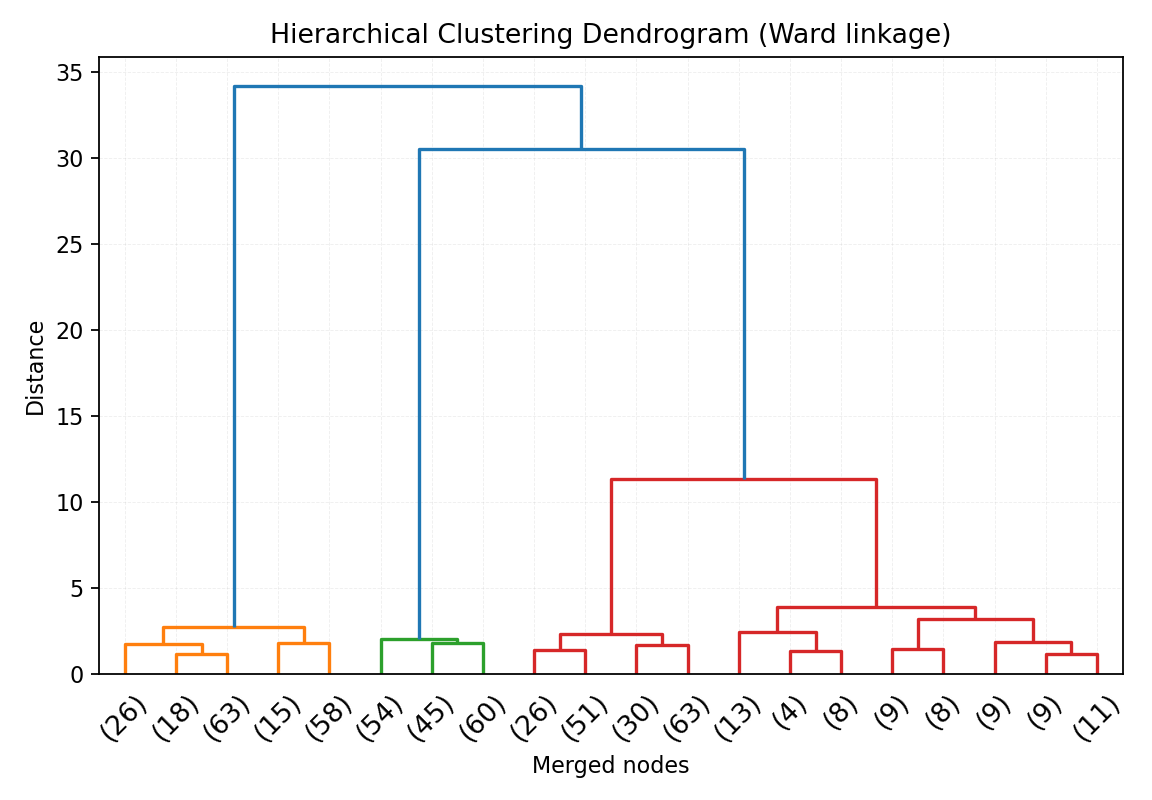
\includegraphics[width=0.85\linewidth]{hierarchical_dendrogram.png}
  \caption{Ward 链接在合成数据上的树状图}
  \label{fig:hierarchical_dendrogram_cn}
\end{figure}

\begin{figure}[H]
  \centering
  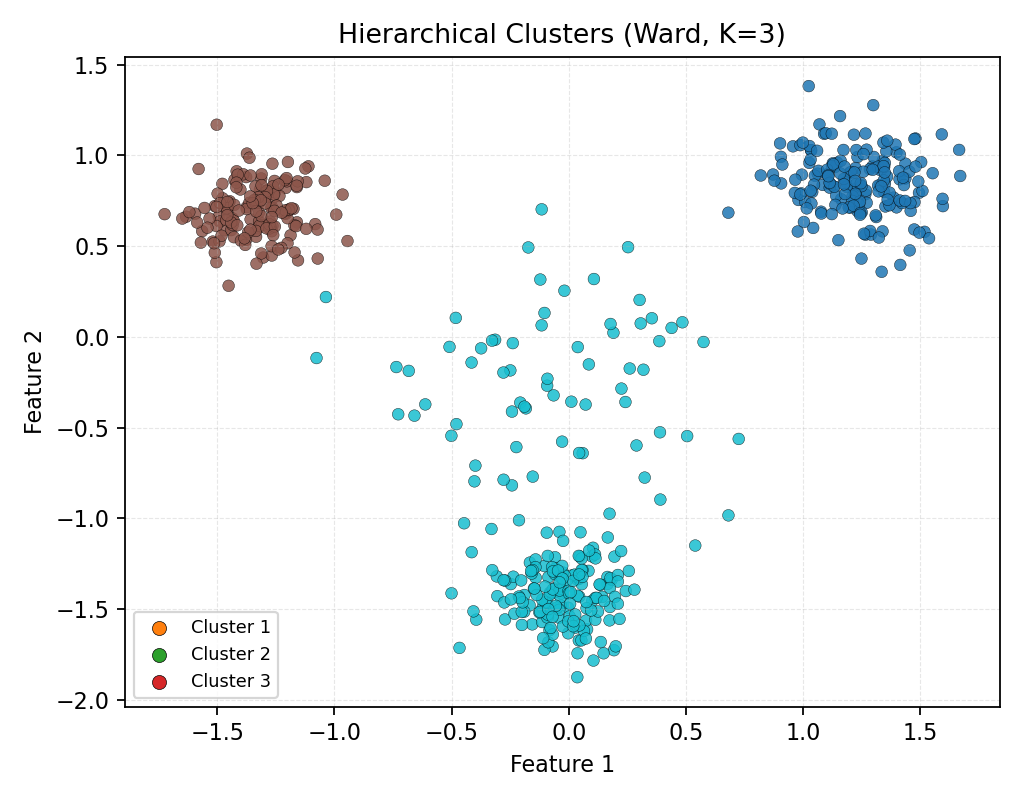
\includegraphics[width=0.82\linewidth]{hierarchical_clusters.png}
  \caption{将树状图切割为三个簇后的二维聚类可视化}
  \label{fig:hierarchical_clusters_cn}
\end{figure}

\FloatBarrier
\section{总结}
层次聚类无需事先指定簇数,适合探索数据的嵌套结构。不同链接方式会影响簇形态:Ward 偏向紧凑簇,average 在链式效应与紧致度之间折中,而 single、complete 强调连通性两端。示例展示了树状图与切割结果如何相辅相成地支持探索分析。

\end{document}
